\section{2 Creating C++ Applications}

Δεν θέλουν όλοι μία υπερ-ανεπτυγμένη GIS εφαρμογή. Μερικές φορές θέλεις απλά να να έχεις ένα απλό widget μέσα στην εφαρμογή σου το οποίο παρουσιάζει ένα χάρτη ενώ ο κύριος στόχος της εφαρμογής να είναι άλλος. Ίσως μία βάση δεδομένων παρουσιασμένος παράλληλα με ένα χάρτη;  Αυτή η ενότητα παρέχει δύο απλά παραδείγματα κώδικα απο τον Tim Sutton, βασισμένα σε προγενέστερη δουλειά του Francis Bolduc. Είναι διαθέσιμα στα αποθετήρια (subversion repositories) του QGIS μαζί με ενδιαφέροντα tutorials. Μπορείτε να ελέγξετε το αποθετήριο στον παρακάτω σύνδεσμο: \filename{https://svn.osgeo.org/qgis/trunk/code\_examples/}

\subsection{2.1 Creating a simple mapping widget}\label{subsec:simple_widget}

With this tutorial we will create a simple mapping widget. It won't do 
anything much - just load a shape file and display it in a random colour. 
This should give you an idea of the potential for using QGIS as an embedded
mapping component.

Θα αρχίσουμε με το να προσθέσουμε τα απαραίτητα συστατικά για την εφαρμογή μας:

\begin{verbatim}
//
// QGIS Includes
//
#include <qgsapplication.h>
#include <qgsproviderregistry.h>
#include <qgssinglesymbolrenderer.h>
#include <qgsmaplayerregistry.h>
#include <qgsvectorlayer.h>
#include <qgsmapcanvas.h>
//
// Qt Includes
//
#include <QString>
#include <QApplication>
#include <QWidget>
\end{verbatim}

Χρησιμοποιούμε το QgsApplication για το QΑpplication του Qt, για να επωφεληθούμε απο τις ποικίλες στατικές μεθόδους που μπορούν να χρησιμοποιηθούν για να εντοπίσουμε τις βιβλιοθήκες και ούτω καθ' εξής. 

Το μητρώο του παροχέα είναι κάτι το μοναδικό που γνωρίζει απο plugin διανυσματικών δεδομένων. Κάνει όλη τη δουλειά για σας φορτώνοντας τα plugin και ούτω καθ' εξής. O renderer του μοναδικού συμβόλου είναι η πιο βασική κλάση συμβολισμού. Κάνει render σε σημεία, γραμμές (polylines) και πολύγωνα σε ένα μοναδικό χρώμα το οποίο επιλέγεται τυχαία εξ'ορισμού (παρ' όλο που μπορείς να το θέσεις μόνος σου). Κάθε επίπεδο διανυσματικής μορφής θα πρέπει να έχει μια συμβολογία με την οποία να σχετίζεται. 

Το μητρώο των επιπέδων του χάρτη “γνωρίζει” όλα τα επίπεδα που χρησιμοποιείτε. Η κλάση του διανυσματικού επιπέδου “κληρονομεί” απο το επίπεδο χάρτη και το επεκτείνει έτσι ώστε να συμπεριλαμβάνει για τα διανυσματικά δεδομένα. 

Εν τέλει, ο κανβάς του χάρτη είναι η κύρια περιοχή του χάρτη μας. Είναι το σχειδιαζόμενο widget πάνω στο οποίο ο χάρτης μας θα εμφανίζεται.

Τώρα μπορούμε να προχωρήσουμε στην έναρξη της εφαρμογής μας...

\begin{verbatim}
int main(int argc, char ** argv)
{
  // Start the Application
  QgsApplication app(argc, argv, true);

  QString myPluginsDir        = "/home/timlinux/apps/lib/qgis";
  QString myLayerPath         = "/home/timlinux/gisdata/brazil/BR_Cidades/";
  QString myLayerBaseName     = "Brasil_Cap";
  QString myProviderName      = "ogr";

\end{verbatim}

Τώρα έχουμε μία  qgsapplication και έχουμε ορίσει μερικές μεταβλητές. Απο τη στιγμή που αυτό το μάθημα αρχικά δοκιμάστηκε σε Ubuntu Linux 8.10, έχουμε ορίσει την θέση του διανυσματικού παροχέα plugin να βρίσκεται μέσα στο φάκελο ανάπτυξης εγκατάστασης. Προφανώς θα είχε περισσότερο νόημα να κρατήσουμε τα QGIS libs σε φάκελο με μια απο τις αρχικές βιβλιοθήκες στο σύστημά σας (π.χ. /usr/lib) αλλά αυτός ο τρόπος είναι επαρκής προς το παρόν. 

Οι επόμενες δύο μεταβλητές που ορίζονται εδώ εστιάζουν στο shape file το οποίο πρόκειται να χρησιμοποιηθεί (παρ' όλο που θα θέλατε να αντικατασήσετε με τα δικά σας δεδομένα εδώ). 

Το όνομα του παροχέα είναι σημαντικό – λέει στο qgis ποιόν παροχέα δεδομένων να χρησιμοποιήσει για να φορτώσει το αρχείο. Τυπικά θα χρησιμοποιήσετε το 'org' ή postgres'

Τώρα μπορούμε να προχωρήσουμε στην ουσιαστική δημιουργία του αντικείμενου του επιπέδου.

\begin{verbatim}
  // Instantiate Provider Registry
  QgsProviderRegistry::instance(myPluginsDir);
\end{verbatim}

Αρχικά βάζουμε τον παροχέα μητρώου να ξεκινήσει. Είναι μια μοναδική κλάση, οπότε καλούμε τη στατική μεταβλητή και την περνάμε στην αναζήτησης του φακέλου του παροχέα lib. Καθώς ξεκινάει θα ψάξει αυτό το φάκελο για παροχέα libs.

Τώρα προχωράμε στη δημιουργία του layer... 

\begin{verbatim}
  QgsVectorLayer * mypLayer =
      new QgsVectorLayer(myLayerPath, myLayerBaseName, myProviderName);
  QgsSingleSymbolRenderer *mypRenderer = new
QgsSingleSymbolRenderer(mypLayer->geometryType());
  QList <QgsMapCanvasLayer> myLayerSet;

  mypLayer->setRenderer(mypRenderer);
  if (mypLayer->isValid())
  {
    qDebug("Layer is valid");
  }
  else
  {
    qDebug("Layer is NOT valid");
  }

  // Add the Vector Layer to the Layer Registry
  QgsMapLayerRegistry::instance()->addMapLayer(mypLayer, TRUE);
  // Add the Layer to the Layer Set
  myLayerSet.append(QgsMapCanvasLayer(mypLayer, TRUE));

\end{verbatim}

TΟ κώδικας είναι αρκετά κατανοήσιμος εδώ. Δημιουργούμε ένα επίπεδο πληροφορίας χρησιμοποιώντας τις μεταβλητές που ορίσαμε νωρίτερα. Έπειτα αναθέτουμε στο επίπεδο ένα renderer. Όταν δημιουργούμε έναν renderer πρέπει να καθορίσουμε τον τύπο γεωμετρίας, το οποίο το κάνουμε ζητώντας απο το διανυσματικό επίπεδο πληροφορίας για τον τύπο γεωμετρίας. Έπειτα προσθέτουμε το επίπεδο πληροφορίας σε ένα σύνολο επιπέδων (layerset) (το οποίο χρησιμοποιείται απο το QgsMapCanvas για να γνωρίζει επίπεδα πληροφορίας να κάνει render και με ποιά σειρά) και στο μητρώο του επιπέδου πληροφορίας χάρτη (maplayer). Στο τέλος σιγουρευόμαστε ότι το επίπεδο θα είναι ορατό. 

Τώρα θα δημιουργήσουμε έναν κανβά του χάρτη πάνω στο οποίο θα σχεδιάσουμε το επίπεδο πληροφορίας.

\begin{verbatim}
  // Create the Map Canvas
  QgsMapCanvas * mypMapCanvas = new QgsMapCanvas(0, 0);
  mypMapCanvas->setExtent(mypLayer->extent());
  mypMapCanvas->enableAntiAliasing(true);
  mypMapCanvas->setCanvasColor(QColor(255, 255, 255));
  mypMapCanvas->freeze(false);
  // Set the Map Canvas Layer Set
  mypMapCanvas->setLayerSet(myLayerSet);
  mypMapCanvas->setVisible(true);
  mypMapCanvas->refresh();

\end{verbatim}

Για άλλη μία φορά δεν υπαρει κάτι δύσκολο εδώ. Δημιουργούμε τον κανβα και μετά θέτουμε τις επεκτάσεις του επιπέδου πληροφορίας μας. Έπειτα “τσιμπάμε” λίγο τον κανβά έτσι ωστε να σχεδιάσουμε πιο λεία διανυσματικά αρχεία (vectors).  Έπειτα θέτουμε το χρώμα του backgroung, “ξεπαγώνουμε” τον κανβά, τον κάνουμε ορατό και το ανανεώνουμε.

\begin{verbatim}
  // Start the Application Event Loop
  return app.exec();
}

\end{verbatim}

Στο τελευταίο βήμα απλά ξεκινάμε τον Qt βρόχο και είμαστε έτοιμοι. Μπορείτε να ελέγξετε, να συνθέσετε και να τρέξετε το παράδειγμα χρησιμοποιώντας το cmake όπως παρακάτω:

\begin{verbatim}
svn co
https://svn.osgeo.org/qgis/trunk/code_examples/1_hello_world_qgis_style
cd 1_hello_world_qgis_style
mkdir build
#optionally specify where your QGIS is installed (should work on all
platforms)
#if your QGIS is installed to /usr or /usr/local you can leave this next step
out
export LIB_DIR=/home/timlinux/apps
cmake ..
make
./timtut1
\end{verbatim}

Όταν το συνθέτουμε και το τρέξουμε κάπως έτσι θα μοιάζει η εφαρμογή μας.:

\begin{figure}[ht]
   \begin{center}
   \caption{Μια απλή C++ εφαρμογή \osxcaption}\label{fig:cpp1_application}\smallskip
   
\includegraphics[clip=true]{cpp1_application}
\end{center}
\end{figure}

\subsection{2.2 Δουλεύοντας με το QgsMapCanvas}

Στην προηγούμενη ενότητα (ενότητα 2.1) δείξαμε πως να χρησιμοποιήσετε το API του QgsMapCanvas για να δημιουργήσετε μια απλή εφαρμογή που φορτώνει ένα shapefile και δείχνει τα σημεία πάνω του. Αλλά πόσο καλός είναι ένας χάρτης με τον οποίο δεν μπορείς να επικοινωνήσεις; 

Σε αυτό το δεύτερο μάθημα θα επεκτείνουμε το προηγούμενο μάθημα κάνοντάς το μια QmainWindow εφαρμογή με μενού, εργαλειοθήκη και περιοχή κανβά.  Σας δείχνουμε πως να χρησιμοποιείτε το QgsMapTool - την κλάση βάση για όλα τα εργαλεία που χρησιμοποιούνται για να αλληλεπιδρούν με τον κανβά του χάρτη. Η εργασία θα παρέχει τέσσερα εικονίδια για την εργαλειοθήκη για να 

\begin{itemize}
 \item προστίθεται ένα επίπεδο χάρτη 
 \item γίνεται ζουμ προς τα μέσα
 \item γίνεται ζουμ προς τα έξω
 \item να είναι δυνατή η μετακίνηση (panning)
\end{itemize}

Στον κατάλογο εργασίας για τον κώδικα του μαθήματος θα βρείτε έναν αριθμό απο αρχεία συμπεριλαμβάνοντας τον πηγαίο κώδικα C++ , εικονίδια και ένα απλό αρχείο με δεδομένα κάτω απο τα δεδομένα.  Υπάρχει επίσης και το .ui αρχείο για το κυρίως παράθυρο. 

\textbf{Σημείωση:} θα χρειαστεί να προσαρμόσετε το .pro αρχείο στον κατάλογο svn παραπάνω, για να ταιριάξει με το σύστημά σας. 

Αφού αρκετός απο τον κώδικα είναι ίδιος με αυτόν του προηγούμενου μαθήματος, θα επικεντρωθούμε στις ιδιαιτερότητες του MapTool -  οι υπόλοιπες απο τις λεπτομέρειες εφαρμογής μπορούν να ερευνηθούν ελέγχοντας τη φόρμα της εργασίας SVN. To QgsMapTool είναι μία κλάση η οποία αλληλεπιδρά με το MapCanvas χρησιμοποιώντας το δείκτη του ποντικιού. Τo QGIS έχει έναν αριθμό απο QgsMapTools εφαρμοσμένα, και μπορείτε να υποδιαιρέσετε την κλάσση του QgsMapTool για να δημιουργήσετε τη δική σας. Στο mainwindow.cpp θα δείτε ότι έχουμε συμπεριλάβει τους αγωγούς για το QgsMapTools κοντά στην αρχή του αρχείου: 

\begin{verbatim}
     //
     // QGIS Map tools
     //
     #include "qgsmaptoolpan.h"
     #include "qgsmaptoolzoom.h"
     //
     // These are the other headers for available map tools 
     // (not used in this example)
     //
     //#include "qgsmaptoolcapture.h"
     //#include "qgsmaptoolidentify.h"
     //#include "qgsmaptoolselect.h"
     //#include "qgsmaptoolvertexedit.h"
     //#include "qgsmeasure.h"
\end{verbatim}

Όπως βλέπετε χρησιμοποιώ μόνο δύο τύπους των υποκλάσεων του MapTool για αυτό το μάθημα, αλλά υπάρχουν περισσότερες διαθέσιμες στη βιβλιοθήκη του QGIS. Συνεοντας τα MapTools στον κανβάς είναι πολύ εύκολο χρησιμοποιώντας τον κανονικό Qt4 signal/slot μηχανισμό: 

\begin{verbatim}
     //create the action behaviours
     connect(mActionPan, SIGNAL(triggered()), this, SLOT(panMode()));
     connect(mActionZoomIn, SIGNAL(triggered()), this, SLOT(zoomInMode()));
     connect(mActionZoomOut, SIGNAL(triggered()), this, SLOT(zoomOutMode()));
     connect(mActionAddLayer, SIGNAL(triggered()), this, SLOT(addLayer()));
\end{verbatim}

Μετά δημιουργούμε μια μικρή εργαλειοθήκη για να κρατάμε τα κουμπιά των εργαλείων. Σημειώστε ότι οι ενέργειες mpAction*  δημιουργήθηκαν σε σχεδιαστή 

\begin{verbatim}
     //create a little toolbar
     mpMapToolBar = addToolBar(tr("File"));
     mpMapToolBar->addAction(mpActionAddLayer);
     mpMapToolBar->addAction(mpActionZoomIn);
     mpMapToolBar->addAction(mpActionZoomOut);
     mpMapToolBar->addAction(mpActionPan);
\end{verbatim}

Τώρα δημιουργούμε τα τρία εργαλεία του χάρτη: 

\begin{verbatim}
     //create the maptools
     mpPanTool = new QgsMapToolPan(mpMapCanvas);
     mpPanTool->setAction(mpActionPan);
     mpZoomInTool = new QgsMapToolZoom(mpMapCanvas, FALSE); // false = in
     mpZoomInTool->setAction(mpActionZoomIn);
     mpZoomOutTool = new QgsMapToolZoom(mpMapCanvas, TRUE ); //true = out
     mpZoomOutTool->setAction(mpActionZoomOut);
\end{verbatim}

Για άλλη μία φορά τίποτα εδώ δεν είναι πολύ μπερδεμένο – δημιουργούμε αντικείμενα εργαλείων, κάθε ένα απο απο τα οποία συνεργάζεται με τον ίδιο κανβα χάρτη και με μία διαφορετική QAction. Όταν ο χρήστης επιλέγει ένα απο τα εικονίδια της εργαλειοθήκης, ορίζεται το ενεργό MapTool για τον κανβας.  Για παράδειγμα όταν ενεργοποιείται το εικονίδιο Pan, κάνουμε το εξής: 

\begin{verbatim}
    void MainWindow::panMode()
    {
       mpMapCanvas->setMapTool(mpPanTool); 
    }
\end{verbatim}

\begin{figure}[ht]
   \begin{center}
   \caption{Η εφαρμογή QmainWindow με ένα μενού, μία εργαλειοθήκη και εναν κανβά
\osxcaption}\label{fig:cpp2_application}\smallskip
   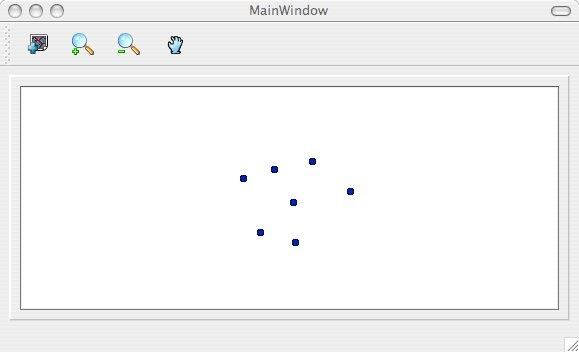
\includegraphics[clip=true, width=12cm]{cpp2_application}
\end{center}
\end{figure}

\minisec{Συμπεράσματα}

Όπως βλέπετε επεκτείνοντας το προηγούμενο παράδειγμα σε κάτι πιο λειτουργικό χρησιμοποιώντας το MapTool είναι πολύ εύκολο και απαιτεί μόνο μερικές γραμμές κώδικα για κάθε MapTool που θέλετε να παρέχετε.

Μπορείτε να ελέγξετε και να γραψετε αυτό το μάθημα χρησιμοποιώντας SVN και Cmake χρησιμοποιώντας τα ακόλουθα βήματα:

\begin{verbatim}
svn co https://svn.osgeo.org/qgis/trunk/code_examples/2_basic_main_window
cd 2_basic_main_window
mkdir build
#optionally specify where your QGIS is installed (should work on all platforms)
#if your QGIS is installed to /usr or /usr/local you can leave this next step out
export LIB_DIR=/home/timlinux/apps
cmake ..
make
./timtut2
\end{verbatim}


